\chapter{Сравнительный анализ моделей}\label{ch3}

В главе \ref{ch3} проводится сравнительный анализ шести моделей, обученных на подготовленных выборках. Цель --- оценить качество предсказания двух ключевых агрономических характеристик: площади покрытия и размера капель. Для обеих задач модели обучались на 80\% данных. Оставшиеся 20\% использовались для тестирования. Результаты сравниваются как по визуальному соответствию предсказаний реальным значениям, так и по метрикам качества --- коэффициенту детерминации $R^2$ (\ref{ch1:R2}) и среднеквадратичной ошибке $RMSE$ (\ref{ch1:RMSE}). Также проводится выявление важнейших признаков, которые внесли наибольший вклад в предсказание целевых переменных.

\section{Предсказание площади покрытия}\label{ch3:coverage}

\subsection{Сравнение результатов предсказаний}

На \firef{fig:coverage-lr} видно, что линейная регрессия не способна точно аппроксимировать зависимости между признаками и покрытием. Предсказания на тестовой выборке значительно отклоняются от истинных значений. Это подтверждается метриками: $R^2 = 0.759$ и $RMSE = 1.29$. Полученные результаты указывают на несоответствие простой линейной модели характеру зависимости в данных, что ожидаемо при высокой размерности пространства признаков.

\begin{figure}[htbp!]
	\centering
	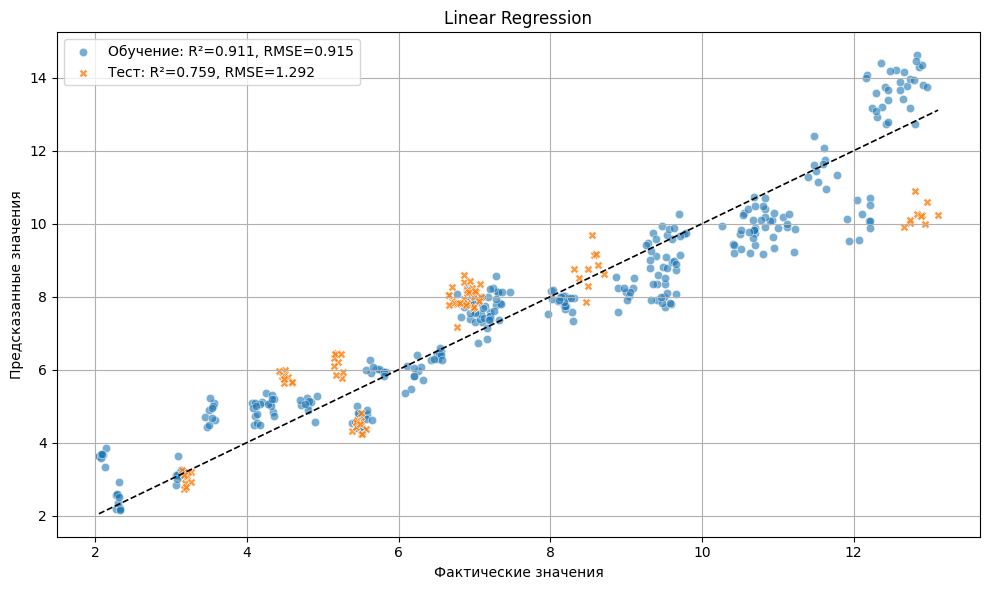
\includegraphics[width=.9\linewidth]{my_folder/images/coverage/Linear-Regression.png}
	\caption{Предсказания линейной регрессии (LR)} 
	\label{fig:coverage-lr}  
\end{figure}

SVR (см. \firef{fig:coverage-svr}), использованный с подобранными параметрами методом поиска на сетке с оценкой через кросс-валидацию, показывает более выраженное приближение на обучении, однако на тестовой выборке наблюдается ухудшение качества предсказаний ($R^2 = 0.699$, $RMSE = 1.44$). Это отражает трудности SVR при работе с разнородными и высокоразмерными данными, несмотря на предварительный подбор гиперпараметров.

\begin{figure}[htbp!]
	\centering
	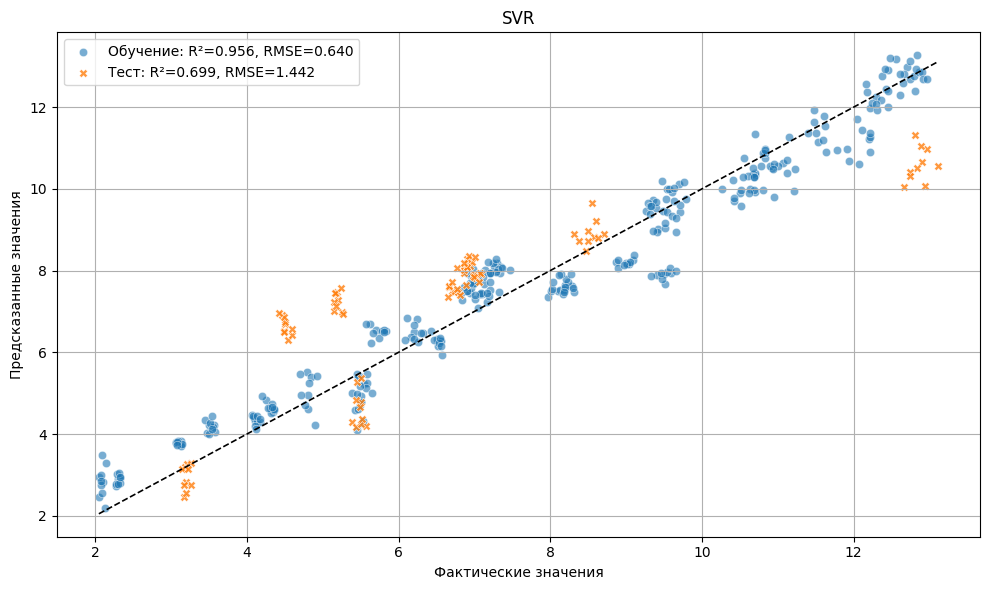
\includegraphics[width=.9\linewidth]{my_folder/images/coverage/SVR.png}
	\caption{Предсказания метода опорных векторов (SVR)} 
	\label{fig:coverage-svr}  
\end{figure}

Случайный лес (см. \firef{fig:coverage-rf}) обеспечивает более высокую точность на обучающей выборке ($R^2 = 0.995$), но на тесте его результат уступает градиентным бустингам, демонстрируя $R^2 = 0.782$ при $RMSE = 1.23$. Несмотря на это, модель остаётся устойчивой.

\begin{figure}[htbp!]
	\centering
	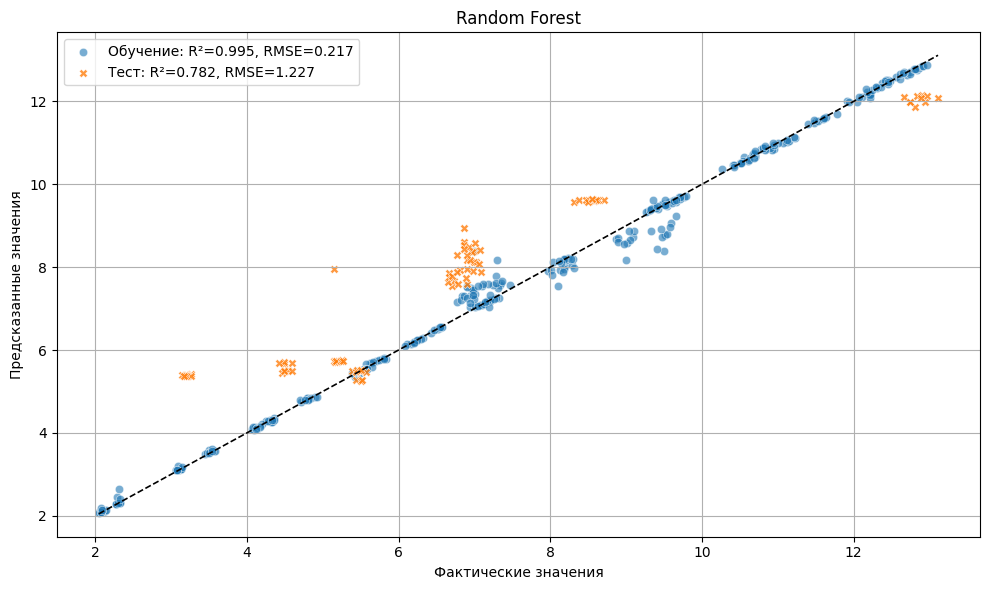
\includegraphics[width=.9\linewidth]{my_folder/images/coverage/Random-Forest.png}
	\caption{Предсказания метода случайного леса (RF)} 
	\label{fig:coverage-rf}  
\end{figure}


Градиентный бустинг (см. \firef{fig:coverage-gbr}) проявил себя надёжно: он уступает CatBoost, но сохраняет высокое качество на тесте ($R^2 = 0.815$, $RMSE = 1.13$), демонстрируя адекватную способность к обобщению сложных зависимостей.

\begin{figure}[htbp!]
	\centering
	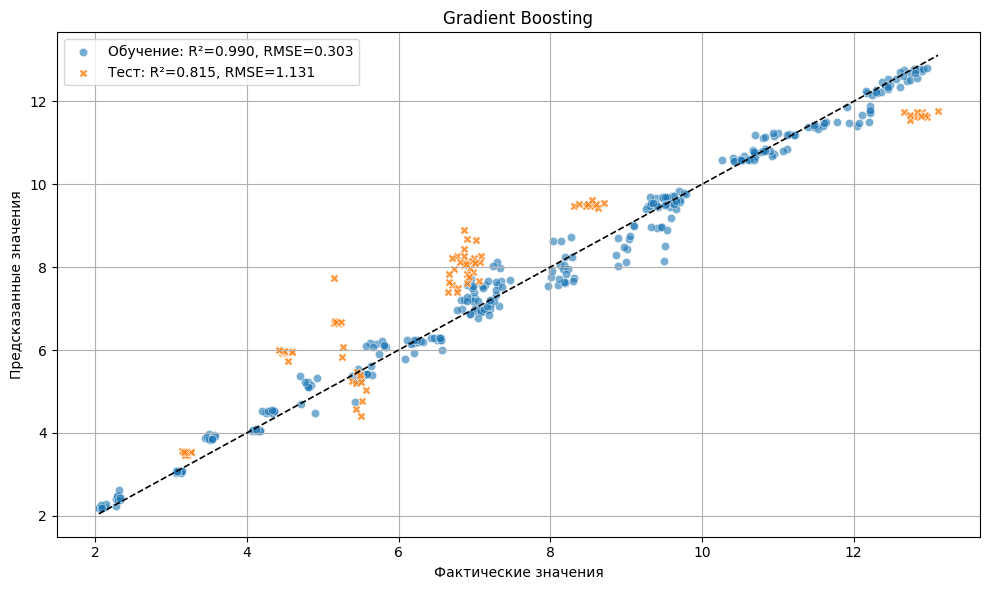
\includegraphics[width=.9\linewidth]{my_folder/images/coverage/Gradient-Boosting.png}
	\caption{Предсказания метода градиентного бустинга (GBR)} 
	\label{fig:coverage-gbr}  
\end{figure}

Использование XGBoost с параметрами по умолчанию приводит к переобучению, что видно по практически идеальному обучающему $R^2 = 0.998$ и заметному падению точности на тесте ($R^2 = 0.793$). Это подчёркивается визуальной расфокусировкой предсказаний на графике (см. \firef{fig:coverage-xgboost-overfit}).

\begin{figure}[htbp!]
	\centering
	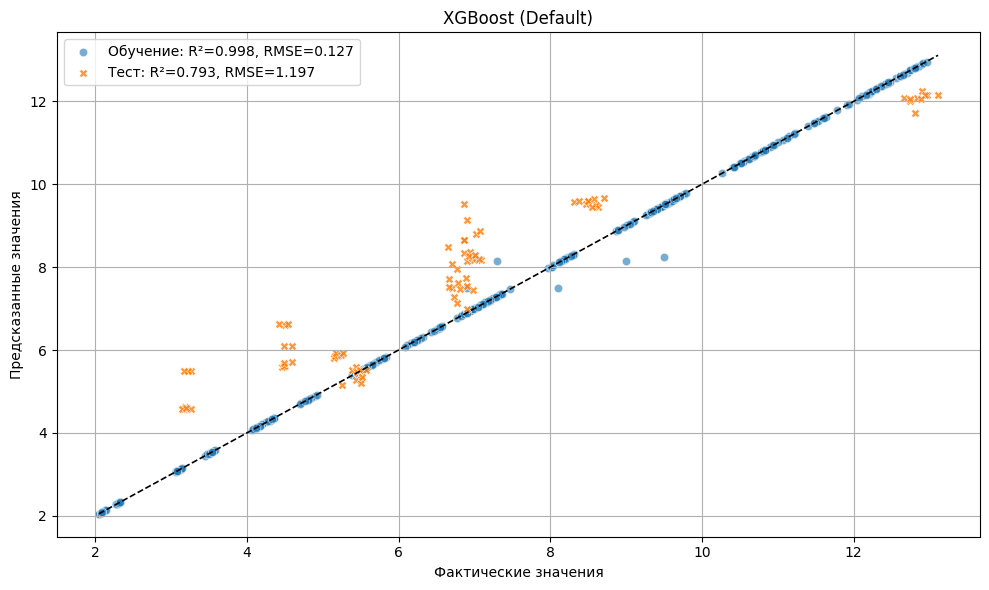
\includegraphics[width=.8\linewidth]{my_folder/images/coverage/XGBoost-overfiting.png}
	\caption{Предсказания XGBoost до настройки параметров} 
	\label{fig:coverage-xgboost-overfit}  
\end{figure}

После настройки с помощью генетического алгоритма модель XGBoost частично смягчила переобучение (см. \firef{fig:coverage-xgboost}): качество на обучении снизилось, но улучшения на тесте практически не наблюдается ($R^2 = 0.792$, $RMSE = 1.20$).


\begin{figure}[htbp!]
	\centering
	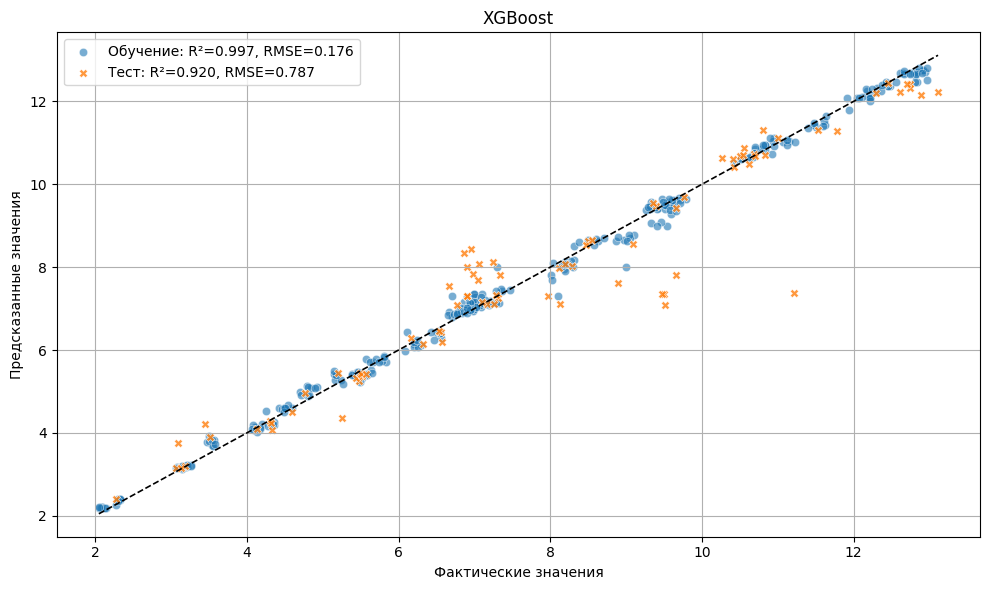
\includegraphics[width=.8\linewidth]{my_folder/images/coverage/XGBoost.png}
	\caption{Предсказания XGBoost после настройки параметров} 
	\label{fig:coverage-xgboost}  
\end{figure}
\newpage


CatBoost продемонстрировал наилучший результат среди всех моделей (см. \firef{fig:coverage-catboost}). Коэффициент детерминации на тестовой выборке составил $R^2 = 0.882$ при $RMSE = 0.90$. Это свидетельствует о высокой устойчивости модели к структурным особенностям данных и сильной способности к обобщению.


\begin{figure}[htbp!]
	\centering
	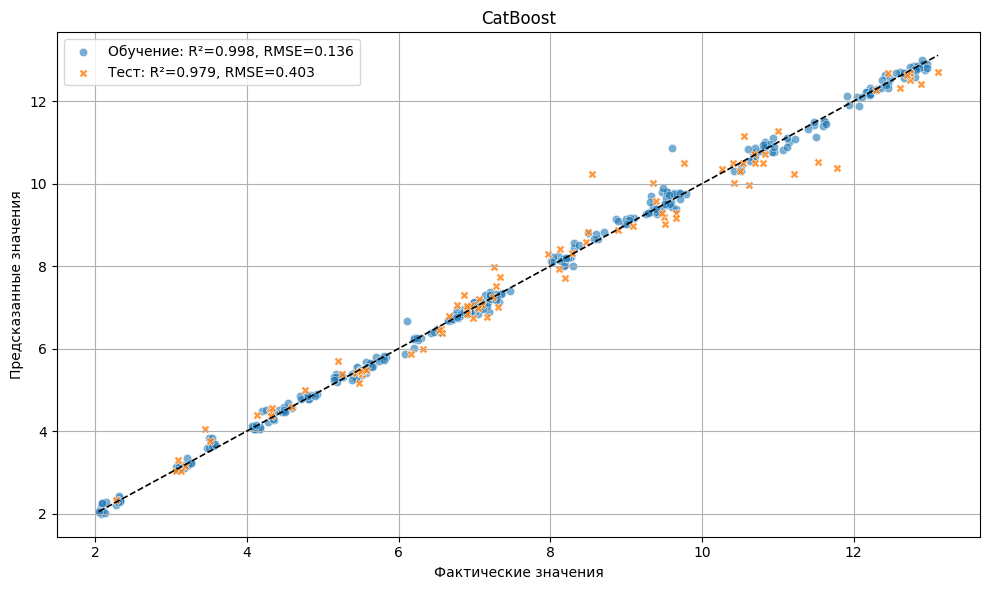
\includegraphics[width=.9\linewidth]{my_folder/images/coverage/CatBoost.png}
	\caption{Предсказания модели CatBoost} 
	\label{fig:coverage-catboost}  
\end{figure}

В \taref{tab:coverage-table} отражены значения метрик для каждой модели:

\begin{table}[htbp!]
	\centering\small
	\caption{Сводная таблица $R^2$ и $RMSE$ для площади покрытия}
	\label{tab:coverage-table}		
	\begin{tabular}{|l|c|c|c|c|}
		\hline
		\multirow{2}{*}{Модель} & \multicolumn{2}{|c|}{Обучающая выборка} & \multicolumn{2}{c|}{Тестовая выборка}\\\cline{2-5} 
		& $R^2$ & $RMSE$ & $R^2$ & $RMSE$\\\hline
		CatBoost&0.998585&0.115213&0.882371&0.901760\\
		GradientBoosting&0.990218&0.302911&0.814927&1.131111\\
		XGBoost (Default)&0.998290&0.126628&0.792790&1.196849\\
		XGBoost (GA-Tuning)&0.994903&0.218646&0.792265&1.198363\\
		RandomForest&0.994976&0.217081&0.782113&1.227295\\
		LinearRegression&0.910811&0.914635&0.758507&1.292069\\
		SVR&0.956363&0.639769&0.699309&1.441762\\
		\hline
	\end{tabular}	
	\normalsize
\end{table}

Они подтверждают высокую устойчивость ансамблевых методов, особенно CatBoost, который демонстрирует наилучшее сочетание точности и обобщающей способности: самый высокий $R^2$ и минимальный $RMSE$ на тестовой выборке. GBR и RF также показывают высокую обучаемость, однако уступают CatBoost по точности на тестовых данных. Модели XGBoost, как в базовой конфигурации, так и после настройки, демонстрируют признаки переобучения. LR и SVR являются наименее эффективными в условиях высокой размерности пространства признаков.

\subsection{Выявление важных признаков}

Рассмотрим, какие признаки оказались наиболее важными для прогнозирования площади покрытия в моделях, показавших лучшие результаты. В модели CatBoost объём распыления даёт 65.5\% суммарной важности, скорость полёта --- 8.0\%, минимальная влажность воздуха --- 3.4\%, а число форсунок --- 2.1\%, тогда как вклад остальных факторов, включая конструктивные характеристики аппарата и оптимальные значения высоты полёта, не превышает 2\%. Соответственно, интенсивность распыления и характеристики окружающего воздуха непосредственно определяют равномерность и площадь покрытия, что согласуется с выводами о том, что высокий объём распыления обеспечивает необходимую плотность осаждения, а скорость влияет на дрейф и покрытие кроны растений \cite{Wu2025}.

В модели GBR: объём распыления --- 76.9\%, минимальная температура воздуха --- 9.4\%, скорость полёта --- 6.8\%, остальные параметры --- не более 1\%.

В модели XGBoost: объём распыления --- 57.6\%, количество форсунок --- 18.5\%, мелкодисперсный режим атомизации --- 7.5\%, минимальная температура --- 6.4\%, объём бака --- 5.8\%, скорость полёта --- 1.7\%, остальные параметры --- не более 0.5\%.

Результаты указывают на то, что необходимо учитывать значимость параметров полёта и метеоусловий для повышения устойчивости прогноза. Кроме того, сформулированный вывод подтверждается работами, использующими компьютерную гидродинамику для моделирования аэродинамики ротора и распределения капель, где скорость полёта, высота и тип форсунок были определены как ключевые факторы равномерного нанесения \cite{Liu2025}, а эмпирические исследования демонстрируют, что параметры распыления и их калибровка существенно влияют на равномерность и эффективность обработки культур \cite{Vitoria2022}. Таким образом, анализ важности признаков для прогнозирования площади покрытия подтвердил, что основными признаками выступают эксплуатационные параметры распыления и метеоусловия. 

\section{Предсказание диаметра капель}\label{ch3:droplet-size}

\subsection{Сравнение результатов предсказаний}

Как и в задаче покрытия, линейная регрессия не смогла качественно справиться с прогнозированием размера капель. На \firef{fig:droplet-size-lr} видно сильное отклонение предсказаний от действительных значений. Метрики подтверждают низкую точность модели ($R = 0.660$, $RMSE = 30.70$).

\begin{figure}[htbp!]
	\centering
	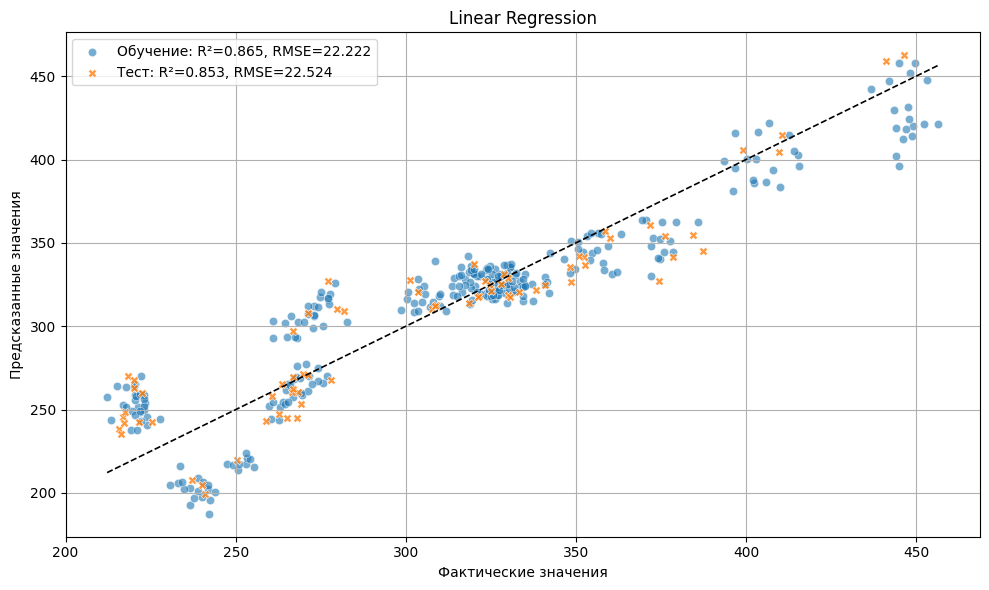
\includegraphics[width=.9\linewidth]{my_folder/images/droplet_size/Linear-Regression.png}
	\caption{Предсказания линейной регрессии (LR)} 
	\label{fig:droplet-size-lr}  
\end{figure}

SVR, несмотря на свою универсальность, также демонстрирует ограниченную обобщающую способность в этой задаче (см. \firef{fig:droplet-size-svr}). $RMSE$ на тесте приблизительно равен $22.96$, а точность составляет лишь $0.810$, что сопоставимо с результатами ансамблевых методов.

\begin{figure}[htbp!]
	\centering
	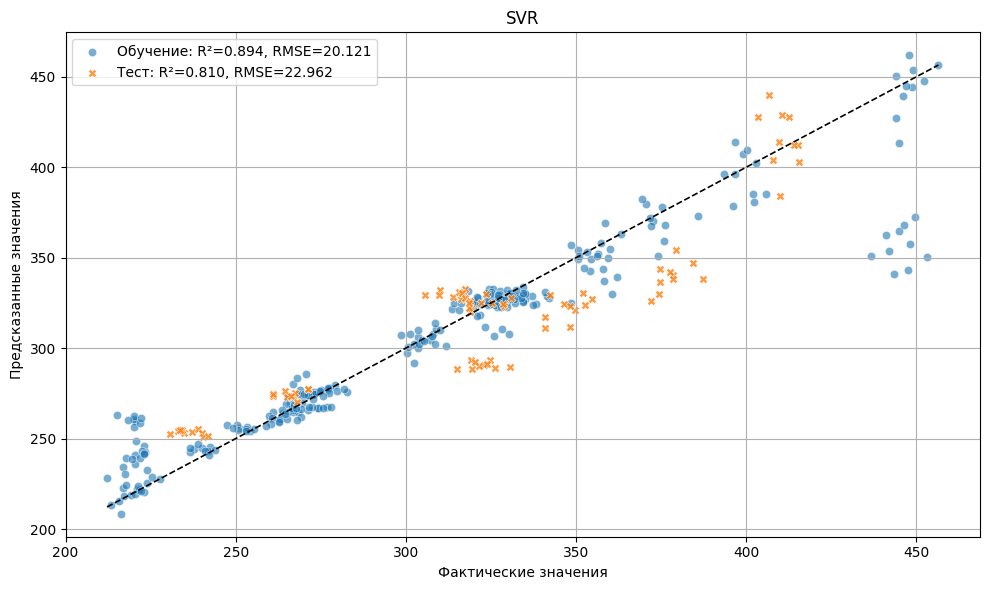
\includegraphics[width=.9\linewidth]{my_folder/images/droplet_size/SVR.png}
	\caption{Предсказания метода опорных векторов (SVR)} 
	\label{fig:droplet-size-svr}  
\end{figure}

Случайный лес (см. \firef{fig:droplet-size-rf}) и градиентный бустинг (см. \firef{fig:droplet-size-gbr}) обеспечили почти схожие результаты ($R^2 = 0.810$, $RMSE = 22.94$ и $R^2 = 0.820$, $RMSE = 22.35$ соответственно), при этом оба метода продемонстрировали неплохую аппроксимацию на обучающей выборке, но незначительное падение точности на тесте.

\begin{figure}[htbp!]
	\centering
	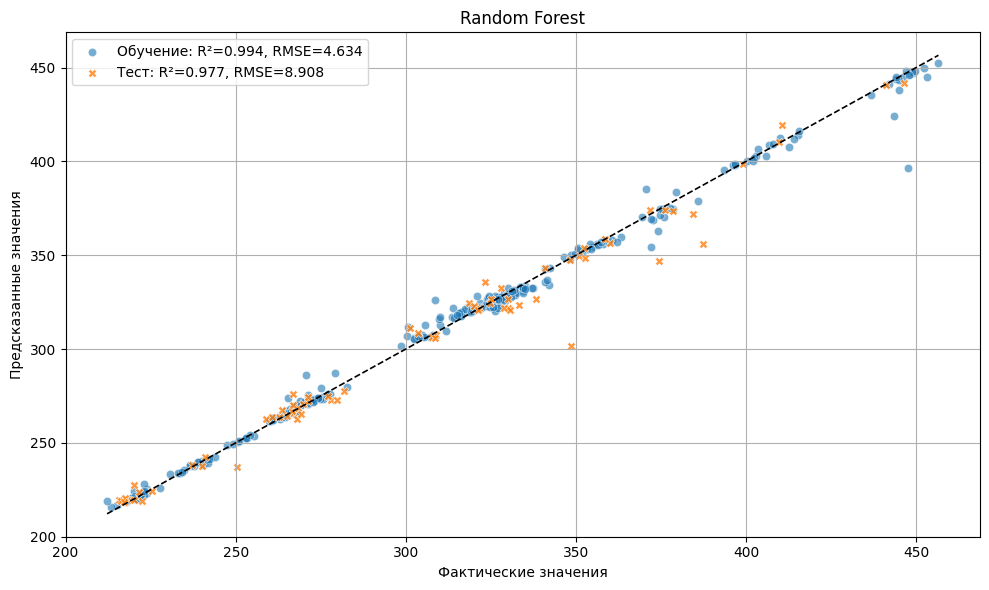
\includegraphics[width=.9\linewidth]{my_folder/images/droplet_size/Random-Forest.png}
	\caption{Предсказания метода случайного леса (RF)} 
	\label{fig:droplet-size-rf}  
\end{figure}


\begin{figure}[htbp!]
	\centering
	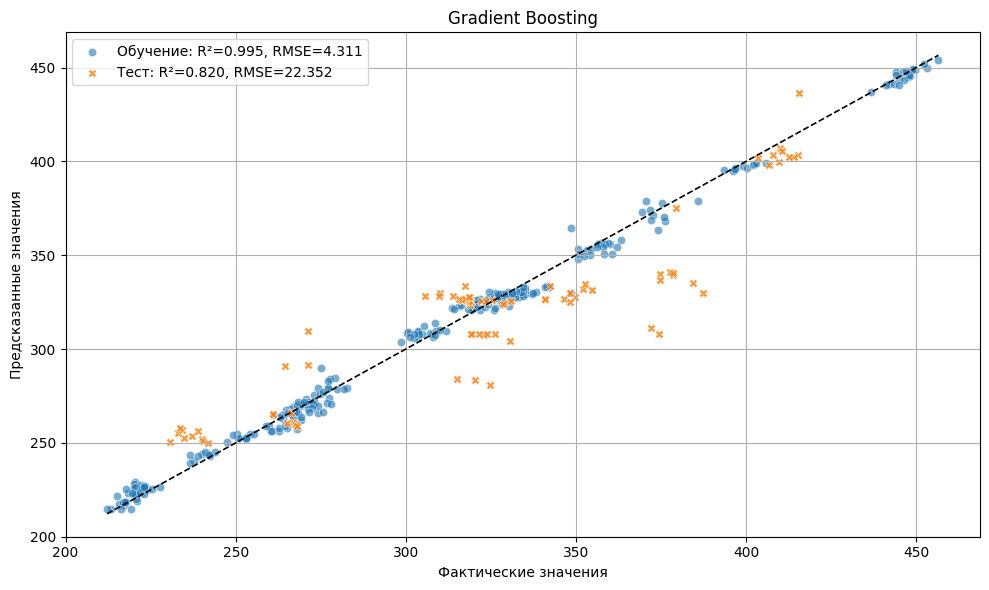
\includegraphics[width=.9\linewidth]{my_folder/images/droplet_size/Gradient-Boosting.png}
	\caption{Предсказания метода градиентного бустинга (GBR)} 
	\label{fig:droplet-size-gbr}  
\end{figure}
\newpage

Для задачи предсказания диаметра капель XGBoost также подвержен переобучению. На \firef{fig:droplet-size-xgboost-overfit} видно почти полное совпадение предсказаний на обучении ($R^2 = 0.9999$, $RMSE = 0.57$), но значительное снижение точности на тесте ($R^2 = 0.863$, $RMSE = 19.47$). Попытка настройки XGBoost с помощью генетического алгоритма (см. \firef{fig:droplet-size-xgboost}) позволила несколько сгладить переобучение, однако общие показатели на тесте ухудшились ($R^2 = 0.811$, $RMSE = 22.90$).

\begin{figure}[htbp!]
	\centering
	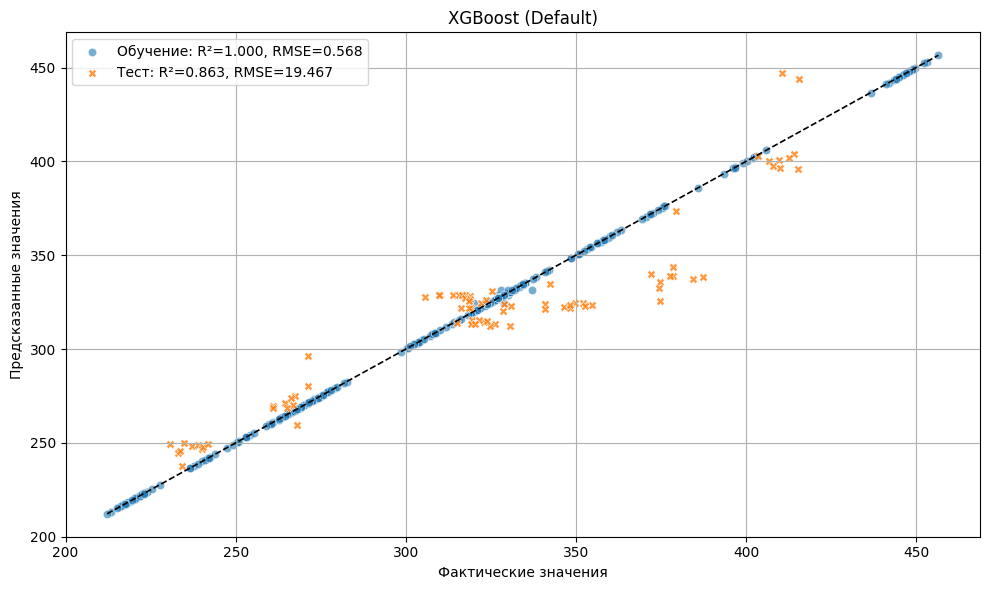
\includegraphics[width=.9\linewidth]{my_folder/images/droplet_size/XGBoost-overfiting.png}
	\caption{Предсказания XGBoost до настройки параметров} 
	\label{fig:droplet-size-xgboost-overfit}  
\end{figure}

\begin{figure}[htbp!]
	\centering
	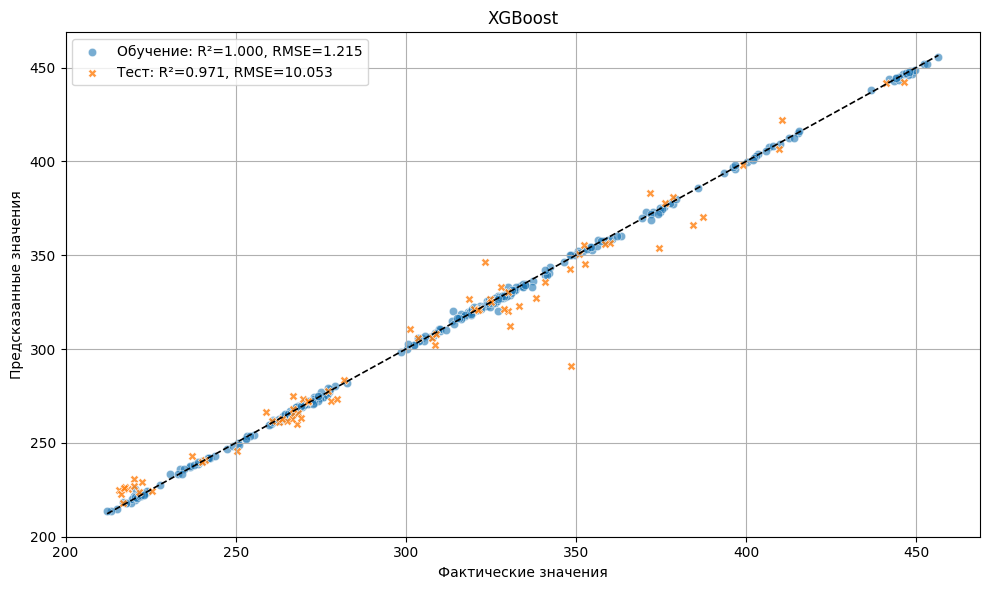
\includegraphics[width=.9\linewidth]{my_folder/images/droplet_size/XGBoost.png}
	\caption{Предсказания XGBoost после настройки параметров} 
	\label{fig:droplet-size-xgboost}  
\end{figure}

\newpage

CatBoost снова показал лучшие результаты, обеспечив наилучшее соотношение точности и ошибки на тестовой выборке (см. \firef{fig:droplet-size-catboost}). При $R^2 = 0.864$ и $RMSE = 19.44$ модель демонстрирует стабильную производительность и умеренное переобучение, что делает её предпочтительным выбором.


\begin{figure}[htbp!]
	\centering
	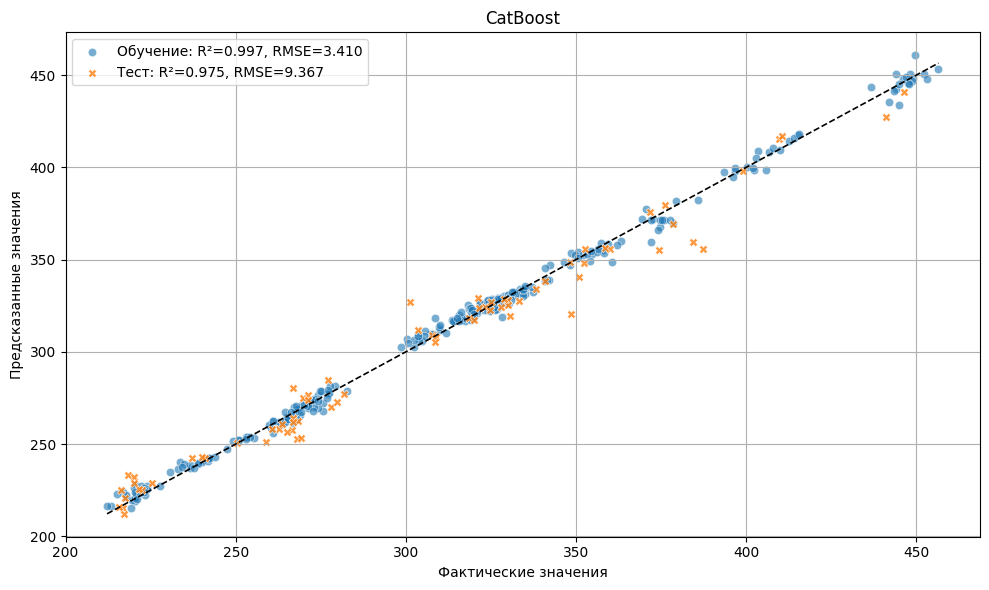
\includegraphics[width=.9\linewidth]{my_folder/images/droplet_size/CatBoost.png}
	\caption{Предсказания модели CatBoost} 
	\label{fig:droplet-size-catboost}  
\end{figure}

В \taref{tab:droplet-size-table} сведены все значения метрик, полученные при предсказании диаметров капель:

\begin{table}[htbp!]
	\centering\small
	\caption{Сводная таблица $R^2$ и $RMSE$ для диаметра капель}
	\label{tab:droplet-size-table}		
	\begin{tabular}{|l|c|c|c|c|}
		\hline
		\multirow{2}{*}{Модель} & \multicolumn{2}{c|}{Обучающая выборка} & \multicolumn{2}{c|}{Тестовая выборка}\\\cline{2-5} 
		& $R^2$ & $RMSE$ & $R^2$ & $RMSE$\\\hline
		CatBoost&0.997282&3.219687&0.863812&19.442279\\
		XGBoost (Default)&0.999915&0.568252&0.863462&19.467204\\
		GradientBoosting&0.995127&4.311346&0.820001&22.351813\\
		XGBoost (GA-Tuning)&0.992029&5.513798&0.811052&22.900683\\
		RandomForest&0.994150&4.723604&0.810464&22.936303\\
		SVR&0.893861&20.120588&0.810034&22.962318\\
		LinearRegression&0.877465&21.618812&0.660338&30.704413\\
		\hline
	\end{tabular}	
	\normalsize
\end{table}

Значения подтверждают, что наилучший результат обеспечил метод CatBoost. RF и GBR показали схожее качество на обучении, однако уступили на тесте. Модель XGBoost в базовой конфигурации достигла высокой точности, но сопровождалась резким ростом переобучения, которое лишь частично удалось смягчить с помощью настройки гиперпараметров. SVR и LR, несмотря на умеренную точность на обучающей выборке, продемонстрировали худшие результаты на тесте.

\subsection{Выявление важных признаков}

Теперь аналогично рассмотрим задачу прогнозирования диаметра капель. В CatBoost объём распыления составляет 55.4\% общей важности, диаметр атомизации --- 13.3\%, высота полёта --- 4.4\%, мощность пропеллеров --- 4.0\%, скорость полёта --- 2.7\%, а количество форсунок --- 2.4\%, что указывает на прямую зависимость размеров капель от объёма подачи, настроек распылительного потока и параметров полёта. Важность остальных признаков не превышает 2\%. 

При этом в XGBoost на первом месте по важности --- мелкодисперсный режим атомизации (35.4\%), за ним следуют объём бака (25.7\%) и крупнодисперсный режим (24.3\%), а объём распыления здесь составляет лишь 13.0\%, что подчёркивает роль точной настройки форсунок для формирования требуемого спектра капель \cite{Liu2025, Vitoria2022}. Остальные признаки составили не более 0.6\% важности.

В модели GBR объём распыления достигает 57.1\%, крупнодисперсный режим атомизации --- 10.5\%, минимальная скорость ветра --- 7.6\%, мелкодисперсный режим --- 6.2\%, объём бака --- 5.7\%, высота полёта --- 3.3\%, скорость полёта --- 2.2\%, остальные признаки --- не более 1.9\%. Это подтверждает сильное влияние как настроек форсунок, так и метеоусловий на размер капель и их траекторию \cite{Liu2025}.

Для задачи прогнозирования диаметра капель самыми важными оказались объём и режимы распыления, хотя структура их вкладов несколько отличается от задачи покрытия. Также не малый вклад внесли аэродинамические факторы.


\section{Выводы}

Проведённый анализ продемонстрировал устойчивое преимущество ансамблевых моделей градиентного бустинга над линейными и простыми нелинейными подходами при решении задач регрессии в условиях агротехнических данных. CatBoost показал наилучшее сочетание точности и устойчивости в обеих задачах, подтверждая свою пригодность для работы с неоднородными и неполными данными. XGBoost, несмотря на высокую точность на обучении, склонен к переобучению, что требует дополнительной настройки или регуляризации. Модели без бустинга, линейная регрессия и SVR, существенно уступают как по точности, так и по устойчивости.

Обобщая результаты важности признаков, можно заключить, что для обеих задач --- как площади покрытия, так и диаметра капель --- параметры объёма распыления и скорость полёта остаются ключевыми. При прогнозировании диаметра капель особое значение приобретает режим атомизации. Также немаловажными оказались число форсунок и объём бака.
